%!TEX root = ../main.tex
\chapter{Statica dei fluidi}

\section{Generalità sui fluidi: densità e pressione}

Si passa ora dallo studio dei solidi, a quello di un fluido, ossia di un materiale in fase liquida o gassosa. Ci si limiterà a studiarne le condizioni di equilibrio statico. Nei corpi in forma solida, i legami molecolari sono talmente forti da rendere difficile deformarli, anche se in realtà essi hanno sempre un grado di deformabilità, tanto che un corpo ha anche proprietà elastiche.

Un materiale indeformabile può essere allungato in maniera elastica, per poi tornare quindi alla posizione di partenza o in maniera plastica e quindi permanente. Sicuramente però quando si va a studiare un fluido c'è una grossa differenza in termini di legami molecolari. Fondamentalmente i fluidi, mentre possono resistere ad un tentativo di compressione, non sono in grado di sopportare gli sforzi di taglio. Se si prende un fluido, gli si può applicare una forza che sia ortogonale alla superficie cercando di comprimerlo e non si comprimerà. Se si va a spingere a lato il fluido, cosa che si traduce dicendo che gli si sta \emph{applicando uno sforzo di taglio}, esso trasla. I fluidi non riescono a opporsi alle forze di taglio e quindi sono messi in movimento. Dal punto di vista microscopico, questo è dovuto al fatto che i legami molecolari tendono ad essere molto deboli nel piano del liquido, quindi si verifica uno scorrimento delle molecole.
Se ci si vuole limitare a studiare un fluido in condizione statiche, bisogna immaginare di essere in una situazione in cui le forze esterne sul fluido sono normali alla superficie, ed entrerà in gioco il concetto di pressione. Presa una superficie $dS$ all'interno del fluido, orientata in maniera casuale, su di essa agirà una forza che dovrà essere necessariamente normale ad essa, altrimenti sarebbe di taglio e metterebbe $dS$ in moto.

\begin{figure}[htpb]
	\centering

	\tikzset{every picture/.style={line width=0.75pt}} %set default line width to 0.75pt        

	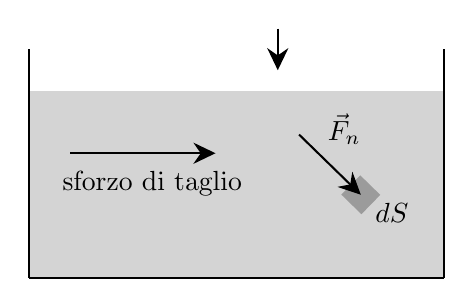
\begin{tikzpicture}[x=0.75pt,y=0.75pt,yscale=-1,xscale=1]
	%uncomment if require: \path (0,300); %set diagram left start at 0, and has height of 300

	%Shape: Rectangle [id:dp3713564616734577] 
	\draw  [draw opacity=0][fill={rgb, 255:red, 212; green, 212; blue, 212 }  ,fill opacity=1 ] (170,130) -- (370,130) -- (370,220) -- (170,220) -- cycle ;
	%Shape: Rectangle [id:dp8448984996265976] 
	\draw  [draw opacity=0][fill={rgb, 255:red, 155; green, 155; blue, 155 }  ,fill opacity=1 ] (329.71,170.63) -- (339.37,180.06) -- (330.29,189.37) -- (320.63,179.94) -- cycle ;
	%Straight Lines [id:da35624833529467814] 
	\draw    (170,110) -- (170,220) ;
	%Straight Lines [id:da9756231879480504] 
	\draw    (370,110) -- (370,220) ;
	%Straight Lines [id:da6992538058902569] 
	\draw    (170,220) -- (370,220) ;
	%Straight Lines [id:da08382077498641105] 
	\draw    (290,100) -- (290,117) ;
	\draw [shift={(290,120)}, rotate = 270] [fill={rgb, 255:red, 0; green, 0; blue, 0 }  ][line width=0.08]  [draw opacity=0] (10.72,-5.15) -- (0,0) -- (10.72,5.15) -- (7.12,0) -- cycle    ;
	%Straight Lines [id:da5990049494414285] 
	\draw    (190,160) -- (257,160) ;
	\draw [shift={(260,160)}, rotate = 180] [fill={rgb, 255:red, 0; green, 0; blue, 0 }  ][line width=0.08]  [draw opacity=0] (10.72,-5.15) -- (0,0) -- (10.72,5.15) -- (7.12,0) -- cycle    ;
	%Straight Lines [id:da2443778154609575] 
	\draw    (300.25,151) -- (327.85,177.91) ;
	\draw [shift={(330,180)}, rotate = 224.27] [fill={rgb, 255:red, 0; green, 0; blue, 0 }  ][line width=0.08]  [draw opacity=0] (10.72,-5.15) -- (0,0) -- (10.72,5.15) -- (7.12,0) -- cycle    ;

	% Text Node
	\draw (229.5,174.5) node   [align=left] {sforzo di taglio};
	% Text Node
	\draw (322,148.5) node    {$\vec{F}_{n}$};
	% Text Node
	\draw (345,188.5) node    {$dS$};

	\end{tikzpicture}
\end{figure}
\FloatBarrier
Questa forza, che si può immaginare per unità di superficie, prende il nome di \textbf{pressione} agente nel fluido in quel punto. È una grandezza scalare, si sa già infatti che è frutto di una forza che agisce ortogonalmente alla superficie, è sufficiente darne il valore.
La pressione $p$ è l'intensità della forza infinitesima che agisce su una superficie infinitesima:

\[
	p(P) = \frac{|d\vec{F}_n|}{dS}
\]

Essa può variare di punto in punto del fluido. Dimensionalmente è una forza per unità di superficie e quindi si misura in: $N/m^2$, a cui si da il nome di \emph{Pascal}, $Pa$. Esistono altre unità di misura molto usate per dare il valore di una pressione. Ad esempio, l'atmosfera è un fluido e ci si aspetta che in ogni punto di essa ci sia una certa pressione. Sulla superficie del mare, essa ha un preciso valore identificato da un'unità di misura che prende il nome di atmosfera:

\[
	1\,atm = 1.013 \times 10^5\,Pa
\]

Altre note unità di misura per la pressione sono:

\begin{itemize}
	\item il bar $1\,bar = 10^5\,Pa$
	\item millimetri di mercurio (in termini di quota di una colonna riempita di mercurio liquido): $1\,atm = 760\,mmHg$
\end{itemize}

Si può dimostrare che la pressione in un fluido, in un certo suo punto, è indipendente da come è orientata la superficie su cui la si sta misurando. Si dice che è una grandezza isotropa, che cioè non dipende appunto da come è orientata la superficie ma soltanto dal punto considerato.

Per caratterizzare un fluido è bene definirne anche la densità. Dato un volumetto di fluido infinitesimo si va a definire la \textbf{densità del fluido} in quel punto come il rapporto:

\[
	p(P) = \frac{dm}{dV} \implies p_{H_2 O, liq } = \frac{1\,kg}{1\,dm^3 } = 10^3\,kg/m^3
\]

\section{Equilibrio statico di un fluido e legge di Stevino}

A questo punto ci si pone come obbiettivo quello di capire come varia la pressione all'interno di un fluido quando è sottoposto all'azione di forze esterne, ad esempio la forza peso. Si otterrà una legge generale che potrà informare su come varia la pressione con la profondità.
Si supponga di avere un fluido in condizioni statiche, cioè tale per cui, preso un volumetto di esso, questo sarà in equilibrio rispetto alle forze che agiscono. Bisogna però distinguere le forze in due categorie:

\begin{itemize}
	\item \textbf{Forze di volume}: quelle forze tali per cui la loro intensità è proporzionale al volume.
	\item \textbf{Forze di superficie}: si tratta di forze che agiscono su ognuna delle faccine del volumetto, la loro intensità è proporzionale alla superficie su cui stanno agendo e sono legate alla pressione del fluido.
\end{itemize}

\begin{figure}[htpb]
	\centering

	\tikzset{every picture/.style={line width=0.75pt}} %set default line width to 0.75pt        

	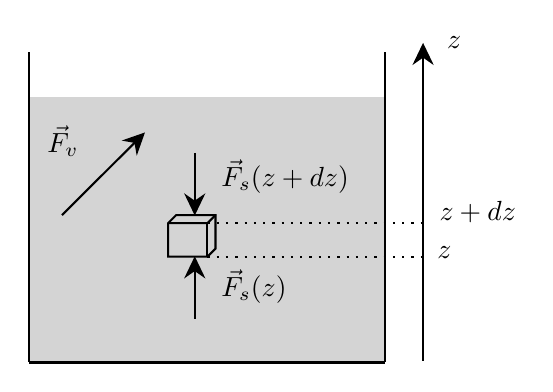
\begin{tikzpicture}[x=0.75pt,y=0.75pt,yscale=-1,xscale=1]
	%uncomment if require: \path (0,300); %set diagram left start at 0, and has height of 300

	%Shape: Rectangle [id:dp7439777710631521] 
	\draw  [draw opacity=0][fill={rgb, 255:red, 212; green, 212; blue, 212 }  ,fill opacity=1 ] (160,143) -- (331.5,143) -- (331.5,271) -- (160,271) -- cycle ;
	%Straight Lines [id:da12104530843999184] 
	\draw    (160,121.58) -- (160,271) ;
	%Straight Lines [id:da7693512673530147] 
	\draw    (331.5,121.58) -- (331.5,271) ;
	%Straight Lines [id:da2919712740516276] 
	\draw    (160,271) -- (331.5,271) ;
	%Straight Lines [id:da8045135759389666] 
	\draw    (240,170) -- (240,197.17) ;
	\draw [shift={(240,200.17)}, rotate = 270] [fill={rgb, 255:red, 0; green, 0; blue, 0 }  ][line width=0.08]  [draw opacity=0] (10.72,-5.15) -- (0,0) -- (10.72,5.15) -- (7.12,0) -- cycle    ;
	%Straight Lines [id:da5794484438449439] 
	\draw    (350,270.1) -- (350,120) ;
	\draw [shift={(350,117)}, rotate = 450] [fill={rgb, 255:red, 0; green, 0; blue, 0 }  ][line width=0.08]  [draw opacity=0] (10.72,-5.15) -- (0,0) -- (10.72,5.15) -- (7.12,0) -- cycle    ;
	%Straight Lines [id:da935822571715307] 
	\draw    (176,200) -- (213.87,162.28) ;
	\draw [shift={(216,160.17)}, rotate = 495.12] [fill={rgb, 255:red, 0; green, 0; blue, 0 }  ][line width=0.08]  [draw opacity=0] (10.72,-5.15) -- (0,0) -- (10.72,5.15) -- (7.12,0) -- cycle    ;
	%Shape: Cube [id:dp6006406406068177] 
	\draw   (227.14,203.89) -- (231.03,200) -- (250,200) -- (250,216.11) -- (246.11,220) -- (227.14,220) -- cycle ; \draw   (250,200) -- (246.11,203.89) -- (227.14,203.89) ; \draw   (246.11,203.89) -- (246.11,220) ;
	%Straight Lines [id:da3179623071123807] 
	\draw    (240,222.83) -- (240,250) ;
	\draw [shift={(240,219.83)}, rotate = 90] [fill={rgb, 255:red, 0; green, 0; blue, 0 }  ][line width=0.08]  [draw opacity=0] (10.72,-5.15) -- (0,0) -- (10.72,5.15) -- (7.12,0) -- cycle    ;
	%Straight Lines [id:da7311859668862664] 
	\draw  [dash pattern={on 0.84pt off 2.51pt}]  (246.11,203.89) -- (350,203.89) ;
	%Straight Lines [id:da042259797735868965] 
	\draw  [dash pattern={on 0.84pt off 2.51pt}]  (246.11,220) -- (350,220) ;

	% Text Node
	\draw (176.5,164.5) node    {$\vec{F}_{v}$};
	% Text Node
	\draw (365,117) node    {$z$};
	% Text Node
	\draw (283.5,181.5) node    {$\vec{F}_{s}( z+dz)$};
	% Text Node
	\draw (268.5,234.5) node    {$\vec{F}_{s}( z)$};
	% Text Node
	\draw (360.33,218) node    {$z$};
	% Text Node
	\draw (376.33,198.67) node    {$z+dz$};

	\end{tikzpicture}
\end{figure}
\FloatBarrier
Si immagini di avere all'interno del fluido una certa forza di volume, che ha una direzione qualunque rispetto a un sistema di riferimento $xyz$ come in figura. Essa ha una componente lungo i tre assi $x, y$ e $z$. La faccia più bassa del volumetto è alla quota $z$, mentre quella più alta alla quota $z+dz$. Si tratta infatti di un volume molto piccolo di lati $dx, dy, dz$. In condizioni di equilibrio statico la forza di superficie, cioè la pressione di tutte le altre parti del fluido, varierà in modo tale da equilibrare la forza di volume.  Si studia ora il problema solo lungo l'asse $z$ per poi generalizzare. Lungo $z$ si avrà una pressione che agisce sulla faccia più alta del volume e una sulla faccia più bassa (analogamente si ha la pressione che agisce nelle altre direzioni). Si impone che le forze totali sul fluido debbano equilibrarsi fra di loro:

\begin{gather*}
	\vec{F}_s + \vec{F}_v = 0 \quad \text{scompongo lungo z}\\
	z:\quad p(z)dS - p(z+dz)dS + F_{v,z} = 0
\end{gather*}
$dS$ è un elemento di superficie che si può scrivere come: $dS=dx\,dy$.
Si definisce la forza di volume che sta agendo in un certo volume del fluido introducendo il concetto di \textbf{densità della forza di volume}. Essa è il rapporto:

\[
	\vec{f}_v = \frac{\vec{F}_v }{dm} \]

Si ha quindi:

\[
	\quad \vec{F}_v = \vec{f}_v\,dm = \vec{f}_v\rho dV = \vec{f}_v\rho\,dx\,dy\,dz
\]

\begin{equation*}
	\begin{aligned}
		z&:\quad p(z)dx\,dy - p(z+dz)dx\,dy + f_v\,dx\,dy\,dz = 0 \\
		z&:\quad p(z) - p(z+dz) + f_v dz = 0
	\end{aligned}
\end{equation*}

Ora bisogna semplicemente riscrivere il secondo termine sfruttando le proprietà delle derivate. La derivata di una funzione infatti non è altro che il limite del rapporto incrementale:

\begin{gather*}
	\frac{dp}{dz} = \frac{p(z+dz)-p(z)}{dz} \implies p(z+dz)=\frac{dp}{dz}dz + p(z) \\
	z:\quad p(z)-p(z) - \frac{dp}{dz}dz + \vec{f}_{v,z}\rho dz =0 \\
	\frac{dp}{dz} = \vec{f}_{v,z}\rho
\end{gather*}

Data una certa direzione, la pressione del fluido varierà con la posizione esattamente in maniera tale da essere pari alla densità della forza di volume per la densità del fluido. Questo risultato è stato ottenuto per la componente in $z$, ma un risultato del tutto analogo (la forza di volume è generale in questo caso) lo si otterrà sulle altre direzioni:

\[
	\frac{\partial p}{\partial z}  = f_{v,z}\rho \qquad \frac{\partial p}{\partial y}  = f_{v,y}\rho \qquad \frac{\partial p}{\partial x}  = f_{v,x}\rho
\]

La pressione in un fluido può variare in $x, y, z$ in maniera tale da seguire l'intensità della componente della forza di volume che agisce sul fluido. Questo viene scritto in modo molto più compatto introducento l'operatore \textbf{gradiente}.  È un operatore (per definizione un vettore) che trasforma una grandezza scalare in una grandezza vettoriale ed è la variazione della funzione scalare a cui è applicato nelle tre direzioni dello spazio, ognuna moltiplicata per il suo versore.  Si dimostra che esso indica la direzione di massima variazione della funzione a cui è applicato. Si scrive anche come \emph{nabla} della grandezza.

\[
	\text{grad}p = \rho \vec{f}_v = \left\{ \begin{array}{r}
	 	\frac{\partial p}{\partial z} = f_{v,z}\rho \\
	 	\frac{\partial p}{\partial y} = f_{v,y}\rho \\
	 	\frac{\partial p}{\partial x} = f_{v,x}\rho
	\end{array} \right.
\]

In maniera compatta la relazione si può scrivere dicendo che in un punto di condizioni statiche, la pressione deve variare da punto a punto in modo tale che il suo gradiente sia equiverso e parallelo alla direzione della forza di volume, e in intensità deve essere pari all'intensità di forza di volume per la densità del fluido.

\[
	\text{grad}p = \underbrace{\vec{\nabla}}_\text{`nabla'} p = \frac{\partial p}{\partial x} \vec{u}_x + \frac{\partial p}{\partial y} \vec{u}_y + \frac{\partial p}{\partial z} \vec{u}_z
\]

\paragraph{Esempio} Si immagini che la forza di volume in questione sia la forza peso.

\[
	\vec{F}_v = dm\,\vec{g} = \rho\,dV\vec{g}  \quad \vec{f}_v = \vec{g} = -g\vec{u}_z
\]

Si va a sostituire quello che si ha in questo caso:

\[
	\vec{\nabla} p = \left\{ \begin{array}{l}
	 	\frac{\partial p}{\partial z} = -\rho\,g \\
	 	\frac{\partial p}{\partial y} = 0 \\
	 	\frac{\partial p}{\partial x} = 0
	\end{array} \right.
\]

Si immagini di avere un fluido in cui si pone l'origine dell'asse $z$ sul pelo dell'acqua in modo tale da vedere come varia la pressione con la profondità del fluido. Essa aumenta perché il volume di fluido deve sopportare il peso di tutta la colonna d'acqua che c'è sopra di lui, altrimenti l'acqua si muoverebbe verso il basso. Se la densità del fluido ha densità costante:

\[
	\int_{p_0 }^{p(z)} dp = \int_0^{-z} -p\,g\,dz= p(-z) - p_0= -\rho g(-z) \implies p(-z) ) p_0 + \rho gz
\]

Questa prende il nome di \textbf{legge di Stevino}. Essa informa su come varia la pressione in un fluido al variare della profondità. La pressione alla profondità $H$ è la pressione che si avrebbe sul pelo libero dell'acqua più $\rho g H$.

\[
	\boxed{p(H) = p_0 + \rho gH}
\]

La pressione è aumentata del peso della colonna di fluido che sta al di sopra del punto considerato.

\begin{figure}[htpb]
	\centering

	\tikzset{every picture/.style={line width=0.75pt}} %set default line width to 0.75pt        

	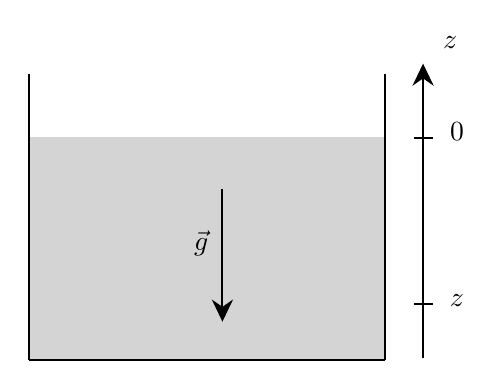
\begin{tikzpicture}[x=0.75pt,y=0.75pt,yscale=-1,xscale=1]
	%uncomment if require: \path (0,300); %set diagram left start at 0, and has height of 300

	%Shape: Rectangle [id:dp9257457317027504] 
	\draw  [draw opacity=0][fill={rgb, 255:red, 212; green, 212; blue, 212 }  ,fill opacity=1 ] (160,135.25) -- (331.5,135.25) -- (331.5,242.67) -- (160,242.67) -- cycle ;
	%Straight Lines [id:da45733836926557014] 
	\draw    (160,105.08) -- (160,242.67) ;
	%Straight Lines [id:da27101038653804976] 
	\draw    (331.5,105.08) -- (331.5,242.67) ;
	%Straight Lines [id:da2452169725190556] 
	\draw    (160,242.67) -- (331.5,242.67) ;
	%Straight Lines [id:da1603614064589991] 
	\draw    (350,242) -- (350,103) ;
	\draw [shift={(350,100)}, rotate = 450] [fill={rgb, 255:red, 0; green, 0; blue, 0 }  ][line width=0.08]  [draw opacity=0] (10.72,-5.15) -- (0,0) -- (10.72,5.15) -- (7.12,0) -- cycle    ;
	%Straight Lines [id:da8367477743150609] 
	\draw    (253.33,160.33) -- (253.33,221.33) ;
	\draw [shift={(253.33,224.33)}, rotate = 270] [fill={rgb, 255:red, 0; green, 0; blue, 0 }  ][line width=0.08]  [draw opacity=0] (10.72,-5.15) -- (0,0) -- (10.72,5.15) -- (7.12,0) -- cycle    ;
	%Straight Lines [id:da6069175472492154] 
	\draw    (345.67,135.67) -- (355,135.67) ;
	%Straight Lines [id:da5622008752683028] 
	\draw    (345.67,215.67) -- (355,215.67) ;

	% Text Node
	\draw (243.17,186.5) node    {$\vec{g}$};
	% Text Node
	\draw (363,90) node    {$z$};
	% Text Node
	\draw (366.33,214) node    {$z$};
	% Text Node
	\draw (366.33,132.67) node    {$0$};

	\end{tikzpicture}
\end{figure}
\FloatBarrier
Si vuole ora capire come varia la pressione con la quota nell'atmosfera. Ci si aspetta che essa diminuisca, perché se si va in quota, sopra si ha una colonna d'aria minore di quella che vi è sopra il pelo dell'acqua. L'atmosfera ha una densità che via via diminuisce mano a mano che ci si sposta in quota e questo rende la relazione è più complicata. Si ha un integrale in cui $\rho$ varia con la quota, la densità dell'aria è proporzionale alla pressione stessa. Si può risolvere e si trova che la $p$ diminuisce esponenzialmente con la quota.

\begin{figure}[htpb]
	\centering

	\tikzset{every picture/.style={line width=0.75pt}} %set default line width to 0.75pt        

	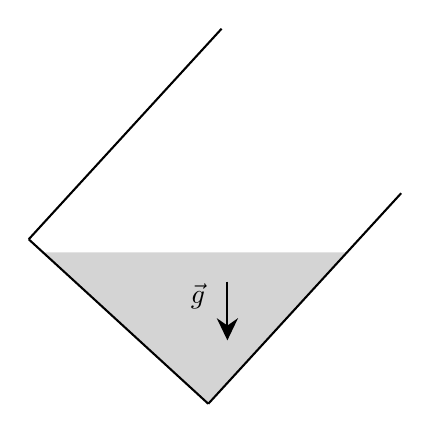
\begin{tikzpicture}[x=0.75pt,y=0.75pt,yscale=-1,xscale=1]
	%uncomment if require: \path (0,300); %set diagram left start at 0, and has height of 300

	%Shape: Polygon [id:ds7354615261716488] 
	\draw  [draw opacity=0][fill={rgb, 255:red, 212; green, 212; blue, 212 }  ,fill opacity=1 ] (252.13,256.9) -- (172.67,183.92) -- (319.33,183.92) -- cycle ;
	%Straight Lines [id:da20099196556604415] 
	\draw    (258.54,76.19) -- (165.61,177.64) ;
	%Straight Lines [id:da2835286186128565] 
	\draw    (345.06,155.44) -- (252.13,256.9) ;
	%Straight Lines [id:da7481027563971243] 
	\draw    (165.61,177.64) -- (252.13,256.9) ;
	%Straight Lines [id:da8587576102155454] 
	\draw    (261.33,198) -- (261.33,223.33) ;
	\draw [shift={(261.33,226.33)}, rotate = 270] [fill={rgb, 255:red, 0; green, 0; blue, 0 }  ][line width=0.08]  [draw opacity=0] (10.72,-5.15) -- (0,0) -- (10.72,5.15) -- (7.12,0) -- cycle    ;

	% Text Node
	\draw (247.17,205.17) node    {$\vec{g}$};

	\end{tikzpicture}
\end{figure}
\FloatBarrier
La legge di Stevino dice che la pressione nel fluido varia massimamente nella direzione in cui sta agendo la forza di volume. Ad esempio, se si ha un bicchiere messo come in figura, il pelo dell'acqua si distribuisce così in conseguenza della legge generale di equilibrio in un fluido. Per non sentire variazione di volume ci si deve muovere ortogonalmente alla forza di volume. Le superfici ortogonali alla forza di volume che sta agendo sono superfici isobare.
Il pelo libero dell'acqua è una superficie isobara. Tutti i suoi punti sono soggetti allo stesso valore della superficie atmosferica. Ecco perché il pelo libero dell'acqua si dispone sempre in modo da essere ortogonale alla forza di volume. Le superfici isobare sono sempre ortogonali all'accelerazione di gravità.

\section{Applicazioni della legge di Stevino}

Ci sono alcuni risultati importanti conseguenza della legge di Stevino.

\paragraph{Legge dei vasi comunicanti} Si hanno due vasi riempiti dello stesso liquido che comunicano tra di loro tramite un tubo: il livello del pelo del liquido, sotto l'ipotesi che sia a contatto con l'atmosfera, sarà lo stesso.

\begin{figure}[htpb]
	\centering

	\tikzset{every picture/.style={line width=0.75pt}} %set default line width to 0.75pt        

	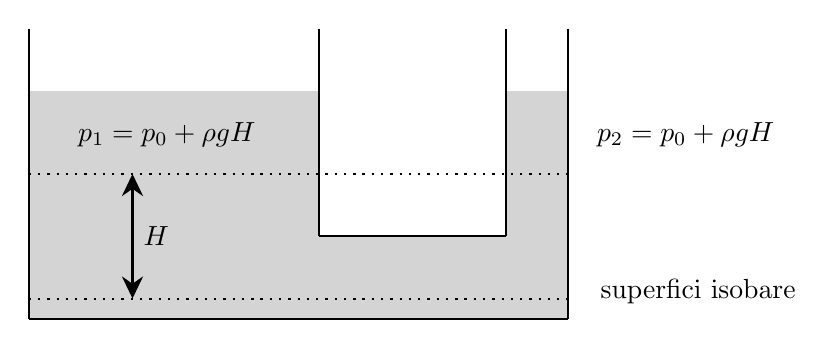
\begin{tikzpicture}[x=0.75pt,y=0.75pt,yscale=-1,xscale=1]
	%uncomment if require: \path (0,300); %set diagram left start at 0, and has height of 300

	%Shape: Rectangle [id:dp27704513154870636] 
	\draw  [draw opacity=0][fill={rgb, 255:red, 212; green, 212; blue, 212 }  ,fill opacity=1 ] (160,130) -- (300,130) -- (300,240) -- (160,240) -- cycle ;
	%Shape: Rectangle [id:dp4584260031687635] 
	\draw  [draw opacity=0][fill={rgb, 255:red, 212; green, 212; blue, 212 }  ,fill opacity=1 ] (390,130) -- (420,130) -- (420,240) -- (390,240) -- cycle ;
	%Shape: Rectangle [id:dp0668709439513262] 
	\draw  [draw opacity=0][fill={rgb, 255:red, 212; green, 212; blue, 212 }  ,fill opacity=1 ] (300,200) -- (390,200) -- (390,240) -- (300,240) -- cycle ;
	%Straight Lines [id:da4468593700445236] 
	\draw    (160,100) -- (160,240) ;
	%Straight Lines [id:da38055217362304306] 
	\draw    (300,100) -- (300,200) ;
	%Straight Lines [id:da049168839863139135] 
	\draw    (160,240) -- (420,240) ;
	%Straight Lines [id:da6961574404465656] 
	\draw    (210,173) -- (210,227) ;
	\draw [shift={(210,230)}, rotate = 270] [fill={rgb, 255:red, 0; green, 0; blue, 0 }  ][line width=0.08]  [draw opacity=0] (10.72,-5.15) -- (0,0) -- (10.72,5.15) -- (7.12,0) -- cycle    ;
	\draw [shift={(210,170)}, rotate = 90] [fill={rgb, 255:red, 0; green, 0; blue, 0 }  ][line width=0.08]  [draw opacity=0] (10.72,-5.15) -- (0,0) -- (10.72,5.15) -- (7.12,0) -- cycle    ;
	%Straight Lines [id:da8280487569760746] 
	\draw    (420,100) -- (420,240) ;
	%Straight Lines [id:da8954022549832723] 
	\draw    (390,100) -- (390,200) ;
	%Straight Lines [id:da05136683391980745] 
	\draw    (390,200) -- (300,200) ;
	%Straight Lines [id:da1644519278898211] 
	\draw    (160,240) -- (420,240) ;
	%Straight Lines [id:da6179116634021047] 
	\draw  [dash pattern={on 0.84pt off 2.51pt}]  (160,170) -- (420,170) ;
	%Straight Lines [id:da16023166347142093] 
	\draw  [dash pattern={on 0.84pt off 2.51pt}]  (160,230) -- (420,230) ;

	% Text Node
	\draw (221.5,200) node    {$H$};
	% Text Node
	\draw (226.5,151) node    {$p_{1} =p_{0} +\rho gH$};
	% Text Node
	\draw (476.5,151) node    {$p_{2} =p_{0} +\rho gH$};
	% Text Node
	\draw (482.5,226.5) node   [align=left] {superfici isobare};

	\end{tikzpicture}
\end{figure}
\FloatBarrier
Infatti, se si considera una superficie ad una certa profondità del fluido, quella superficie tratteggiata deve essere isobara. Ma il salto di pressione tra la pressione nel punto considerato e la superficie, è dato dalla colonna alta $H$ di fluido, quindi le due altezze devono essere uguali. Questo oggetto lo si potrebbe disegnare come un \emph{manometro} a U, che serve per misurare la densità di un fluido rispetto ad un altro di densità nota. Riempiendolo con due liquidi immiscibili, di densità $\rho_1$ e $\rho_2$, i peli si dispongono in maniera tale da non essere più alla stessa quota. Il liquido di densità minore ha bisogno del peso di una colonna più alta.

\begin{figure}[htpb]
	\centering

	\tikzset{every picture/.style={line width=0.75pt}} %set default line width to 0.75pt        

	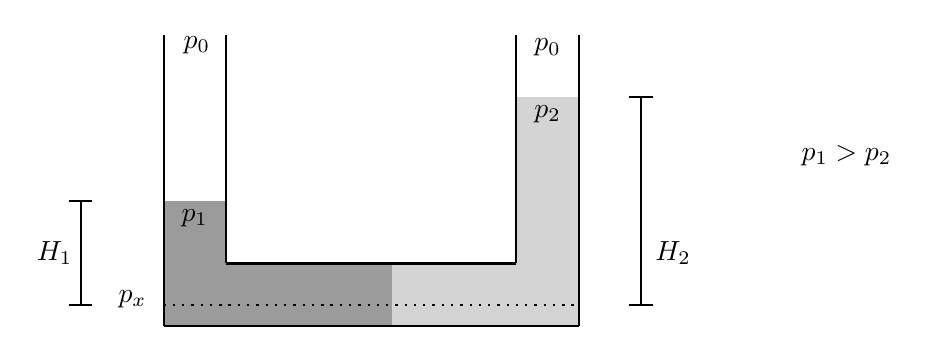
\begin{tikzpicture}[x=0.75pt,y=0.75pt,yscale=-1,xscale=1]
	%uncomment if require: \path (0,300); %set diagram left start at 0, and has height of 300

	%Shape: Rectangle [id:dp44840532884233686] 
	\draw  [draw opacity=0][fill={rgb, 255:red, 212; green, 212; blue, 212 }  ,fill opacity=1 ] (270,210) -- (330,210) -- (330,240) -- (270,240) -- cycle ;
	%Shape: Rectangle [id:dp7423661924962384] 
	\draw  [draw opacity=0][fill={rgb, 255:red, 212; green, 212; blue, 212 }  ,fill opacity=1 ] (330,130) -- (360,130) -- (360,240) -- (330,240) -- cycle ;
	%Shape: Rectangle [id:dp7738438895244188] 
	\draw  [draw opacity=0][fill={rgb, 255:red, 155; green, 155; blue, 155 }  ,fill opacity=1 ] (270,210) -- (270,240) -- (190,240) -- (190,210) -- cycle ;
	%Shape: Rectangle [id:dp9832647459808672] 
	\draw  [draw opacity=0][fill={rgb, 255:red, 155; green, 155; blue, 155 }  ,fill opacity=1 ] (160,180) -- (190,180) -- (190,240) -- (160,240) -- cycle ;
	%Straight Lines [id:da4591492750465662] 
	\draw    (160,100) -- (160,240) ;
	%Straight Lines [id:da3814059419644684] 
	\draw    (190,100) -- (190,210) ;
	%Straight Lines [id:da7914670550753795] 
	\draw    (160,240) -- (360,240) ;
	%Straight Lines [id:da1987832309048725] 
	\draw    (360,100) -- (360,240) ;
	%Straight Lines [id:da31302221508785455] 
	\draw    (330,100) -- (330,210) ;
	%Straight Lines [id:da009014055394372722] 
	\draw    (330,210) -- (190,210) ;
	%Straight Lines [id:da10964146931263641] 
	\draw    (160,240) -- (360,240) ;
	%Straight Lines [id:da6091679957128837] 
	\draw  [dash pattern={on 0.84pt off 2.51pt}]  (160,230) -- (360,230) ;
	%Straight Lines [id:da27691635574222273] 
	\draw    (120,180) -- (120,230) ;
	\draw [shift={(120,230)}, rotate = 270] [color={rgb, 255:red, 0; green, 0; blue, 0 }  ][line width=0.75]    (0,5.59) -- (0,-5.59)   ;
	\draw [shift={(120,180)}, rotate = 270] [color={rgb, 255:red, 0; green, 0; blue, 0 }  ][line width=0.75]    (0,5.59) -- (0,-5.59)   ;
	%Straight Lines [id:da8085267888906842] 
	\draw    (390,130) -- (390,230) ;
	\draw [shift={(390,230)}, rotate = 270] [color={rgb, 255:red, 0; green, 0; blue, 0 }  ][line width=0.75]    (0,5.59) -- (0,-5.59)   ;
	\draw [shift={(390,130)}, rotate = 270] [color={rgb, 255:red, 0; green, 0; blue, 0 }  ][line width=0.75]    (0,5.59) -- (0,-5.59)   ;

	% Text Node
	\draw (145,227) node    {$p_{x}$};
	% Text Node
	\draw (175,188) node    {$p_{1}$};
	% Text Node
	\draw (176,105) node    {$p_{0}$};
	% Text Node
	\draw (345,106) node    {$p_{0}$};
	% Text Node
	\draw (345,138) node    {$p_{2}$};
	% Text Node
	\draw (107.5,205) node    {$H_{1}$};
	% Text Node
	\draw (489,158) node    {$p_{1}  >p_{2}$};
	% Text Node
	\draw (405.5,205) node    {$H_{2}$};

	\end{tikzpicture}
\end{figure}
\FloatBarrier
Per capire la densità $\rho_1$ si guarda la differenza di quota.

\[
	p_x = p_0 + \rho_1 g H_1 = p_0 + \rho_2 gH_2 \implies \boxed{\rho_2 = \rho_1\frac{H_1 }{H_2 }  }
\]

Questa volta si riempie il manometro a U con un fluido di densità nota, l'acqua. Un braccio lo si mette a contatto con l'atmosfera e l'altro con una camera contenente un fluido non miscibile con quello nel manometro.

\begin{figure}[htpb]
	\centering

	\tikzset{every picture/.style={line width=0.75pt}} %set default line width to 0.75pt        

	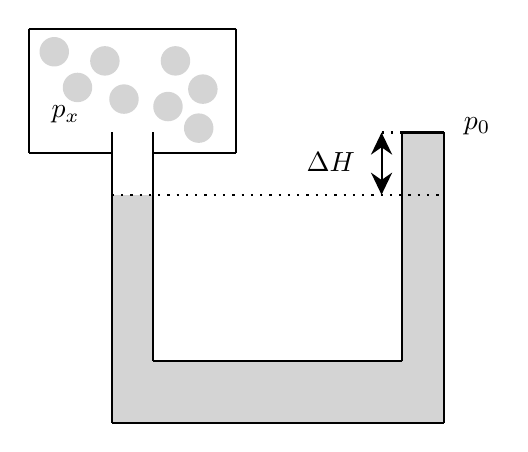
\begin{tikzpicture}[x=0.75pt,y=0.75pt,yscale=-1,xscale=1]
	%uncomment if require: \path (0,300); %set diagram left start at 0, and has height of 300

	%Shape: Rectangle [id:dp3959953820308113] 
	\draw  [draw opacity=0][fill={rgb, 255:red, 212; green, 212; blue, 212 }  ,fill opacity=1 ] (160,130) -- (180,130) -- (180,240) -- (160,240) -- cycle ;
	%Shape: Rectangle [id:dp02069253486010303] 
	\draw  [draw opacity=0][fill={rgb, 255:red, 212; green, 212; blue, 212 }  ,fill opacity=1 ] (180,210) -- (300,210) -- (300,240) -- (180,240) -- cycle ;
	%Shape: Rectangle [id:dp24772278939984171] 
	\draw  [draw opacity=0][fill={rgb, 255:red, 212; green, 212; blue, 212 }  ,fill opacity=1 ] (300,100) -- (320,100) -- (320,240) -- (300,240) -- cycle ;
	%Straight Lines [id:da1464620974589843] 
	\draw    (160,100) -- (160,240) ;
	%Straight Lines [id:da5521606911463739] 
	\draw    (180,100) -- (180,210) ;
	%Straight Lines [id:da3987971312365681] 
	\draw    (160,240) -- (320,240) ;
	%Straight Lines [id:da7965655478878608] 
	\draw    (320,100) -- (320,240) ;
	%Straight Lines [id:da39133260111362134] 
	\draw    (300,100) -- (300,210) ;
	%Straight Lines [id:da5089136574199133] 
	\draw    (300,210) -- (180,210) ;
	%Straight Lines [id:da2020120424295544] 
	\draw    (160,240) -- (320,240) ;
	%Straight Lines [id:da21354002102079073] 
	\draw  [dash pattern={on 0.84pt off 2.51pt}]  (160,130) -- (320,130) ;
	%Straight Lines [id:da5797138891459994] 
	\draw    (320,100) -- (300,100) ;
	%Straight Lines [id:da5184545696166589] 
	\draw  [dash pattern={on 0.84pt off 2.51pt}]  (290,100) -- (320,100) ;
	%Straight Lines [id:da39132803166157104] 
	\draw    (290,103) -- (290,127) ;
	\draw [shift={(290,130)}, rotate = 270] [fill={rgb, 255:red, 0; green, 0; blue, 0 }  ][line width=0.08]  [draw opacity=0] (10.72,-5.15) -- (0,0) -- (10.72,5.15) -- (7.12,0) -- cycle    ;
	\draw [shift={(290,100)}, rotate = 90] [fill={rgb, 255:red, 0; green, 0; blue, 0 }  ][line width=0.08]  [draw opacity=0] (10.72,-5.15) -- (0,0) -- (10.72,5.15) -- (7.12,0) -- cycle    ;
	%Straight Lines [id:da1952310583687571] 
	\draw    (120,50) -- (120,110) ;
	%Straight Lines [id:da9633082911892565] 
	\draw    (220,50) -- (220,110) ;
	%Straight Lines [id:da49174603564191055] 
	\draw    (120,50) -- (220,50) ;
	%Straight Lines [id:da20105406269485737] 
	\draw    (120,110) -- (160,110) ;
	%Straight Lines [id:da4127788726192494] 
	\draw    (180,110) -- (220,110) ;
	%Shape: Circle [id:dp20478396804391652] 
	\draw  [draw opacity=0][fill={rgb, 255:red, 212; green, 212; blue, 212 }  ,fill opacity=1 ] (125.2,61.1) .. controls (125.2,57.18) and (128.38,54) .. (132.3,54) .. controls (136.22,54) and (139.4,57.18) .. (139.4,61.1) .. controls (139.4,65.02) and (136.22,68.2) .. (132.3,68.2) .. controls (128.38,68.2) and (125.2,65.02) .. (125.2,61.1) -- cycle ;
	%Shape: Circle [id:dp5800302968048918] 
	\draw  [draw opacity=0][fill={rgb, 255:red, 212; green, 212; blue, 212 }  ,fill opacity=1 ] (149.6,65.5) .. controls (149.6,61.58) and (152.78,58.4) .. (156.7,58.4) .. controls (160.62,58.4) and (163.8,61.58) .. (163.8,65.5) .. controls (163.8,69.42) and (160.62,72.6) .. (156.7,72.6) .. controls (152.78,72.6) and (149.6,69.42) .. (149.6,65.5) -- cycle ;
	%Shape: Circle [id:dp08611580268843988] 
	\draw  [draw opacity=0][fill={rgb, 255:red, 212; green, 212; blue, 212 }  ,fill opacity=1 ] (136.4,78.3) .. controls (136.4,74.38) and (139.58,71.2) .. (143.5,71.2) .. controls (147.42,71.2) and (150.6,74.38) .. (150.6,78.3) .. controls (150.6,82.22) and (147.42,85.4) .. (143.5,85.4) .. controls (139.58,85.4) and (136.4,82.22) .. (136.4,78.3) -- cycle ;
	%Shape: Circle [id:dp3107456928013643] 
	\draw  [draw opacity=0][fill={rgb, 255:red, 212; green, 212; blue, 212 }  ,fill opacity=1 ] (158.8,83.9) .. controls (158.8,79.98) and (161.98,76.8) .. (165.9,76.8) .. controls (169.82,76.8) and (173,79.98) .. (173,83.9) .. controls (173,87.82) and (169.82,91) .. (165.9,91) .. controls (161.98,91) and (158.8,87.82) .. (158.8,83.9) -- cycle ;
	%Shape: Circle [id:dp957081040610827] 
	\draw  [draw opacity=0][fill={rgb, 255:red, 212; green, 212; blue, 212 }  ,fill opacity=1 ] (183.6,65.5) .. controls (183.6,61.58) and (186.78,58.4) .. (190.7,58.4) .. controls (194.62,58.4) and (197.8,61.58) .. (197.8,65.5) .. controls (197.8,69.42) and (194.62,72.6) .. (190.7,72.6) .. controls (186.78,72.6) and (183.6,69.42) .. (183.6,65.5) -- cycle ;
	%Shape: Circle [id:dp8412082706771953] 
	\draw  [draw opacity=0][fill={rgb, 255:red, 212; green, 212; blue, 212 }  ,fill opacity=1 ] (196.8,79.1) .. controls (196.8,75.18) and (199.98,72) .. (203.9,72) .. controls (207.82,72) and (211,75.18) .. (211,79.1) .. controls (211,83.02) and (207.82,86.2) .. (203.9,86.2) .. controls (199.98,86.2) and (196.8,83.02) .. (196.8,79.1) -- cycle ;
	%Shape: Circle [id:dp8823666291882055] 
	\draw  [draw opacity=0][fill={rgb, 255:red, 212; green, 212; blue, 212 }  ,fill opacity=1 ] (180,87.5) .. controls (180,83.58) and (183.18,80.4) .. (187.1,80.4) .. controls (191.02,80.4) and (194.2,83.58) .. (194.2,87.5) .. controls (194.2,91.42) and (191.02,94.6) .. (187.1,94.6) .. controls (183.18,94.6) and (180,91.42) .. (180,87.5) -- cycle ;
	%Shape: Circle [id:dp2598521058646015] 
	\draw  [draw opacity=0][fill={rgb, 255:red, 212; green, 212; blue, 212 }  ,fill opacity=1 ] (194.8,97.9) .. controls (194.8,93.98) and (197.98,90.8) .. (201.9,90.8) .. controls (205.82,90.8) and (209,93.98) .. (209,97.9) .. controls (209,101.82) and (205.82,105) .. (201.9,105) .. controls (197.98,105) and (194.8,101.82) .. (194.8,97.9) -- cycle ;

	% Text Node
	\draw (137.8,91.4) node    {$p_{x}$};
	% Text Node
	\draw (265.5,114) node    {$\Delta H$};
	% Text Node
	\draw (336,97) node    {$p_{0}$};

	\end{tikzpicture}
\end{figure}
\FloatBarrier
Si vuole capire quale sia la pressione $p_x$. Il fluido si dispone in modo tale da far avere uno sbilanciamento fra i due bracci pari a $\Delta H$. $p_x$ sarà maggiore di $p_o$ perché anche nell'altro braccio alla stessa quota si avrà la stessa pressione di $p_x$, e questa quota sta sotto $p_0$.

\[
	p_x = p_0 + \rho g\Delta H
\]

\paragraph{Il barometro di torricelli} Si ha un recipiente riempito di mercurio. Si usa questo materiale perché è un liquido dalla densità moto elevata. Ora si considera un capillare molto lungo, sopra chiuso e sotto aperto. Si immagina di aspirare completamente tutta l'atmosfera che c'è nel capillare, si dice realizzare il vuoto dentro il capillare. All'intero di esso c'è pressione di 0 $Pa$. Si immerge immediatamente il capillare nel mercurio. Esso risucchia quest'ultimo perché sul pelo del mercurio c'è una pressione atmosferica, alta, che manda il mercurio a riempire il capillare fino ad una certa quota, esattamente pari a 760mm.

\begin{figure}[htpb]
	\centering

	\tikzset{every picture/.style={line width=0.75pt}} %set default line width to 0.75pt        

	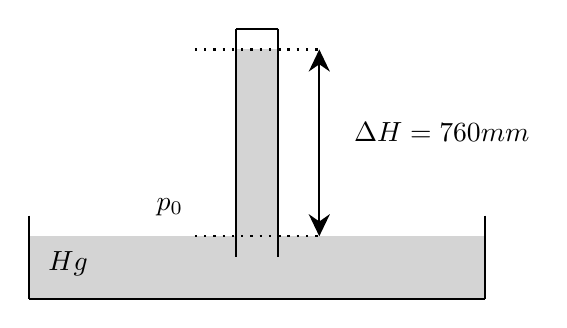
\begin{tikzpicture}[x=0.75pt,y=0.75pt,yscale=-1,xscale=1]
	%uncomment if require: \path (0,300); %set diagram left start at 0, and has height of 300

	%Shape: Rectangle [id:dp4663593906154735] 
	\draw  [draw opacity=0][fill={rgb, 255:red, 212; green, 212; blue, 212 }  ,fill opacity=1 ] (230,110) -- (250,110) -- (250,210) -- (230,210) -- cycle ;
	%Shape: Rectangle [id:dp5997570980829663] 
	\draw  [draw opacity=0][fill={rgb, 255:red, 212; green, 212; blue, 212 }  ,fill opacity=1 ] (130,200) -- (350,200) -- (350,230) -- (130,230) -- cycle ;
	%Straight Lines [id:da38362604979167303] 
	\draw    (130,190) -- (130,230) ;
	%Straight Lines [id:da06020640806887423] 
	\draw    (230,100) -- (230,210) ;
	%Straight Lines [id:da6687943667253919] 
	\draw    (130,230) -- (350,230) ;
	%Straight Lines [id:da4050142485373689] 
	\draw    (350,190) -- (350,230) ;
	%Straight Lines [id:da049442261547041566] 
	\draw    (250,100) -- (250,210) ;
	%Straight Lines [id:da6671297622804289] 
	\draw  [dash pattern={on 0.84pt off 2.51pt}]  (210,110) -- (270,110) ;
	%Straight Lines [id:da8928874617764384] 
	\draw    (270,113) -- (270,197) ;
	\draw [shift={(270,200)}, rotate = 270] [fill={rgb, 255:red, 0; green, 0; blue, 0 }  ][line width=0.08]  [draw opacity=0] (10.72,-5.15) -- (0,0) -- (10.72,5.15) -- (7.12,0) -- cycle    ;
	\draw [shift={(270,110)}, rotate = 90] [fill={rgb, 255:red, 0; green, 0; blue, 0 }  ][line width=0.08]  [draw opacity=0] (10.72,-5.15) -- (0,0) -- (10.72,5.15) -- (7.12,0) -- cycle    ;
	%Straight Lines [id:da20014899847149237] 
	\draw    (230,100) -- (250,100) ;
	%Straight Lines [id:da5254081865605136] 
	\draw  [dash pattern={on 0.84pt off 2.51pt}]  (210,200) -- (270,200) ;

	% Text Node
	\draw (329,150) node    {$\Delta H=760mm$};
	% Text Node
	\draw (198,186) node    {$p_{0}$};
	% Text Node
	\draw (149,213) node    {$Hg$};

	\end{tikzpicture}
\end{figure}
\FloatBarrier
La pressione atmosferica è allora pari al peso di una colonnina di Mercurio alta 760mm.

\[
	\rho g\Delta H + 0 \,atm = p_0 \implies p_0 = \rho g\Delta H
\]

A partire da questo risultato, si utilizzano i $mmHg$ come unità di misura per la pressione.

All'interno del questo concetto espresso dalla legge di Stevino è contenuto il \textbf{principio di Pascal}. Esso afferma che se si applica una variazione di pressione sul fluido, essa si propaga inalterata in tutti i suoi punti.

\paragraph{La pressa idraulica} Si può utilizzare tale principio per realizzare la cosiddetta pressa idraulica. Essa è un oggetto che si utilizza per moltiplicare l'intensità di una forza, al fine ad esempio di sollevare o caricare carichi molto pesanti.

\begin{figure}[htpb]
	\centering

	\tikzset{every picture/.style={line width=0.75pt}} %set default line width to 0.75pt        

	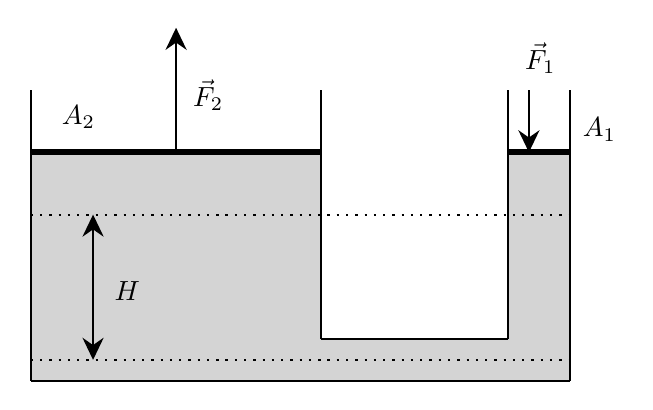
\begin{tikzpicture}[x=0.75pt,y=0.75pt,yscale=-1,xscale=1]
	%uncomment if require: \path (0,300); %set diagram left start at 0, and has height of 300

	%Shape: Rectangle [id:dp3367893604283956] 
	\draw  [draw opacity=0][fill={rgb, 255:red, 212; green, 212; blue, 212 }  ,fill opacity=1 ] (160,130) -- (300,130) -- (300,240) -- (160,240) -- cycle ;
	%Shape: Rectangle [id:dp4131208207535777] 
	\draw  [draw opacity=0][fill={rgb, 255:red, 212; green, 212; blue, 212 }  ,fill opacity=1 ] (390,130) -- (420,130) -- (420,240) -- (390,240) -- cycle ;
	%Shape: Rectangle [id:dp1340729136265908] 
	\draw  [draw opacity=0][fill={rgb, 255:red, 212; green, 212; blue, 212 }  ,fill opacity=1 ] (300,220) -- (390,220) -- (390,240) -- (300,240) -- cycle ;
	%Straight Lines [id:da7123106707750482] 
	\draw    (160,100) -- (160,240) ;
	%Straight Lines [id:da6483304733188897] 
	\draw    (300,100) -- (300,220) ;
	%Straight Lines [id:da5551274557326262] 
	\draw    (160,240) -- (420,240) ;
	%Straight Lines [id:da4554982630064912] 
	\draw    (190,163) -- (190,227) ;
	\draw [shift={(190,230)}, rotate = 270] [fill={rgb, 255:red, 0; green, 0; blue, 0 }  ][line width=0.08]  [draw opacity=0] (10.72,-5.15) -- (0,0) -- (10.72,5.15) -- (7.12,0) -- cycle    ;
	\draw [shift={(190,160)}, rotate = 90] [fill={rgb, 255:red, 0; green, 0; blue, 0 }  ][line width=0.08]  [draw opacity=0] (10.72,-5.15) -- (0,0) -- (10.72,5.15) -- (7.12,0) -- cycle    ;
	%Straight Lines [id:da797810460779933] 
	\draw    (420,100) -- (420,240) ;
	%Straight Lines [id:da24408752045223792] 
	\draw    (390,100) -- (390,220) ;
	%Straight Lines [id:da9437332171240931] 
	\draw    (390,220) -- (300,220) ;
	%Straight Lines [id:da8620671123863763] 
	\draw    (160,240) -- (420,240) ;
	%Straight Lines [id:da5713717636782858] 
	\draw  [dash pattern={on 0.84pt off 2.51pt}]  (160,160) -- (420,160) ;
	%Straight Lines [id:da7323275755860827] 
	\draw  [dash pattern={on 0.84pt off 2.51pt}]  (160,230) -- (420,230) ;
	%Straight Lines [id:da518096766255123] 
	\draw [line width=2.25]    (160,130) -- (300,130) ;
	%Straight Lines [id:da7470580939680109] 
	\draw [line width=2.25]    (390,130) -- (420,130) ;
	%Straight Lines [id:da11589481225675469] 
	\draw    (230,73) -- (230,130) ;
	\draw [shift={(230,70)}, rotate = 90] [fill={rgb, 255:red, 0; green, 0; blue, 0 }  ][line width=0.08]  [draw opacity=0] (10.72,-5.15) -- (0,0) -- (10.72,5.15) -- (7.12,0) -- cycle    ;
	%Straight Lines [id:da9690223161704998] 
	\draw    (400,100) -- (400,127) ;
	\draw [shift={(400,130)}, rotate = 270] [fill={rgb, 255:red, 0; green, 0; blue, 0 }  ][line width=0.08]  [draw opacity=0] (10.72,-5.15) -- (0,0) -- (10.72,5.15) -- (7.12,0) -- cycle    ;

	% Text Node
	\draw (206.5,197) node    {$H$};
	% Text Node
	\draw (183,113) node    {$A_{2}$};
	% Text Node
	\draw (434,119) node    {$A_{1}$};
	% Text Node
	\draw (245.5,102.5) node    {$\vec{F}_{2}$};
	% Text Node
	\draw (405.5,84.5) node    {$\vec{F}_{1}$};

	\end{tikzpicture}
\end{figure}
\FloatBarrier
È un macchinario molto utilizzato nelle officine meccaniche per sollevare le automobili.  Si ha una specie di capillare a U in cui uno dei due bracci ha una sezione molto più piccola dell'altra. Si riempie il capillare di un certo fluido di densità nota. A questo punto i due bracci sono in equilibrio perché su entrambi agisce la pressione atmosferica. Ad un certo punto si applica a sinistra una forza $\vec{F}_1$ che è equivalente ad applicare una variazione di pressione pari a $\norm{\vec{F}_1}/A_1$. Questa variazione di pressione si propaga inalterata in tutti i punti del fluido, fino al braccio destro. Si avrà a destra una forza $\vec{F}_2$ moltiplicata di un fattore proporzionale al rapporto fra le due aree. Il risultato è che il meccanico spinge sul pedale applicando una forza non troppo forte, che viene moltiplica di un fattore molto alto pari al rapporto tra l'area $A_2$ e $A_1$, riuscendo così a sollevare l'automobile.

\[
	p_0+ \frac{F_1 }{A_1 } = p_0 + \frac{F_2 }{A_2 } \qquad F_2 = F_1\frac{A_2 }{A_1 } \quad (\gg F_1 )
\]

Questo aumento della forza è andato a scapito del fatto che il meccanico ha spinto sul pedale andando ad abbassare la colonnina di fluido di un $\Delta x_1$ molto maggiore di quanto si è sollevato il pistone su cui è la macchina, per la conservazione della massa. Deve essere valido:

\[
	A_1\Delta x_1 = A_2\Delta x_2
\]

perché se spingendo il pedale il volume di fludio nel braccio a sinistra diminuisce di una certa quantità, della stessa quantità deve poi aumentare nel braccio di destra.

Il lavoro della forza $\vec{F}_1$ è esattamente uguale a quello fatto dalla $\vec{F}_2$.

\[
	\mathcal{L}_{F_1 } = F_1 \Delta x_1 \quad \mathcal{L}_{F_2 } = F_2 \Delta x_2 = \underbrace{F_1\frac{A_2}{A_1} }_{F_2} \underbrace{\frac{A_1}{A_2}\Delta x_1}_{\Delta x_2 } = F_1 \Delta x_1 = \mathcal{L}_{F_1}
\]

\paragraph{Superfici isobare e superfici equipotenziali} Si è visto che il gradiente della pressione è sempre diretto come la forza di volume che sta agendo. Se ad esempio il fluido è soggetto soltanto alla forza peso, per cui la forza di volume per unità di massa non è altro che l'accelerazione di gravità, la pressione dovrà variare spostandosi verso il fondo del recipiente. Questo perché le superfici ortogonali al gradiente della pressione sono isobare. È importante notare che l'energia potenziale associata alla forza peso è $mgz$, che aumenta con la quota. La superfici equipotenziali sono allora le superfici a $z$ costante. Si potrebbe dimostrare che quando si ha un fluido in condizioni statiche le superficie isobare sono anche equipotenziali. Non vale solo nel caso della forza peso ma anche in quello in cui la forza di volume è un'altra.

Si immagini di avere un bicchiere in condizioni statiche e di metterlo su un carrellino, che si muove di moto accelerato uniforme.

\begin{figure}[htpb]
	\centering

	\tikzset{every picture/.style={line width=0.75pt}} %set default line width to 0.75pt        

	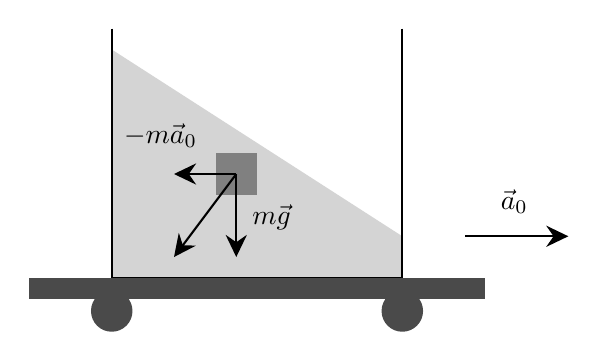
\begin{tikzpicture}[x=0.75pt,y=0.75pt,yscale=-1,xscale=1]
	%uncomment if require: \path (0,300); %set diagram left start at 0, and has height of 300

	%Shape: Polygon [id:ds5968286621281482] 
	\draw  [draw opacity=0][fill={rgb, 255:red, 212; green, 212; blue, 212 }  ,fill opacity=1 ] (300,220) -- (300,240) -- (160,240) -- (160,130) -- cycle ;
	%Straight Lines [id:da8695446790694943] 
	\draw    (160,120) -- (160,240) ;
	%Straight Lines [id:da6436112391399056] 
	\draw    (300,120) -- (300,240) ;
	%Straight Lines [id:da4690519581967658] 
	\draw    (160,240) -- (300,240) ;
	%Straight Lines [id:da3136281429797212] 
	\draw    (377,220) -- (330,220) ;
	\draw [shift={(380,220)}, rotate = 180] [fill={rgb, 255:red, 0; green, 0; blue, 0 }  ][line width=0.08]  [draw opacity=0] (10.72,-5.15) -- (0,0) -- (10.72,5.15) -- (7.12,0) -- cycle    ;
	%Shape: Rectangle [id:dp7713581388669724] 
	\draw  [draw opacity=0][fill={rgb, 255:red, 74; green, 74; blue, 74 }  ,fill opacity=1 ] (120,240) -- (340,240) -- (340,250) -- (120,250) -- cycle ;
	%Shape: Circle [id:dp5064776968626046] 
	\draw  [draw opacity=0][fill={rgb, 255:red, 74; green, 74; blue, 74 }  ,fill opacity=1 ] (150,256) .. controls (150,250.48) and (154.48,246) .. (160,246) .. controls (165.52,246) and (170,250.48) .. (170,256) .. controls (170,261.52) and (165.52,266) .. (160,266) .. controls (154.48,266) and (150,261.52) .. (150,256) -- cycle ;
	%Shape: Circle [id:dp47319546248089894] 
	\draw  [draw opacity=0][fill={rgb, 255:red, 74; green, 74; blue, 74 }  ,fill opacity=1 ] (290,256) .. controls (290,250.48) and (294.48,246) .. (300,246) .. controls (305.52,246) and (310,250.48) .. (310,256) .. controls (310,261.52) and (305.52,266) .. (300,266) .. controls (294.48,266) and (290,261.52) .. (290,256) -- cycle ;
	%Shape: Rectangle [id:dp4245897025459362] 
	\draw  [draw opacity=0][fill={rgb, 255:red, 128; green, 128; blue, 128 }  ,fill opacity=1 ] (210,180) -- (230,180) -- (230,200) -- (210,200) -- cycle ;
	%Straight Lines [id:da0738617207736405] 
	\draw    (220,227) -- (220,190) ;
	\draw [shift={(220,230)}, rotate = 270] [fill={rgb, 255:red, 0; green, 0; blue, 0 }  ][line width=0.08]  [draw opacity=0] (10.72,-5.15) -- (0,0) -- (10.72,5.15) -- (7.12,0) -- cycle    ;
	%Straight Lines [id:da25227835718417047] 
	\draw    (191.8,227.6) -- (220,190) ;
	\draw [shift={(190,230)}, rotate = 306.87] [fill={rgb, 255:red, 0; green, 0; blue, 0 }  ][line width=0.08]  [draw opacity=0] (10.72,-5.15) -- (0,0) -- (10.72,5.15) -- (7.12,0) -- cycle    ;
	%Straight Lines [id:da579938384724676] 
	\draw    (193,190) -- (220,190) ;
	\draw [shift={(190,190)}, rotate = 0] [fill={rgb, 255:red, 0; green, 0; blue, 0 }  ][line width=0.08]  [draw opacity=0] (10.72,-5.15) -- (0,0) -- (10.72,5.15) -- (7.12,0) -- cycle    ;

	% Text Node
	\draw (354,203.5) node    {$\vec{a}_{0}$};
	% Text Node
	\draw (237,211) node    {$m\vec{g}$};
	% Text Node
	\draw (183.5,171.5) node    {$-m\vec{a}_{0}$};

	\end{tikzpicture}
\end{figure}
\FloatBarrier
Si può sfruttare il concetto di sistemi di riferimento non inerziali. Si immagini di osservare quello che succede al fluido dal punto di vista di un osservatore posto sopra il carrellino, e che quindi accelera con esso: per lui tale fluido è fermo. Un elemento di fluido di volume $dV$ e massa $dm$ sarà soggetto alle forze reali (la forza peso $dm\,g$) e alle forze apparenti legate al fatto che il sistema di riferimento accelera in avanti. Ogni massa del fluido sarà soggetta a una forza di volume pari alla somma vettoriale dell'accelerazione di gravità e $-a_o$. In tal caso nel bicchiere il gradiente della pressione dovrà variare esattamente in questa direzione, sarà parallelo ed equiverso alla forza di volume per unità di massa. La superficie libera dell'acqua diventa quella in figura.

\paragraph{Liquido in rotazione} Esattamente lo stesso discorso si può applicare se invece il bicchiere lo si fa ruotare rispetto ad un asse $z$ di simmetria del fluido. Nasce un vettore velocità angolare diretto verso l'alto, che si immagina costante.
Considerato un elemento infinitesimo generico del fluido, esso è soggetto all'accelerazione di gravità e ad una forza centrifuga diretta verso l'esterno pari a $\omega_0 2r$ (dove $r$ e la distanza dell'elemento di fluido dall'asse).
Mentre l'azione dell'accelerazione di gravità è la stessa su tutti i volumetti del fluido, l'accelerazione centrifuga è diversa in ogni punto. Mano a mano che ci si allontana dall'asse l'accelerazione centrifuga aumenta. Si ha un esempio in cui la forza totale di volume varia in direzione e in intensità di punto a punto. Anche il gradiente non cambia mano a mano che ci si sposta nei punti del fluido. Il pelo libero dell'acqua, in conseguenza a questa situazione, assume la forma che si osserva in figura.

\begin{figure}[htpb]
	\centering

	\tikzset{every picture/.style={line width=0.75pt}} %set default line width to 0.75pt        

	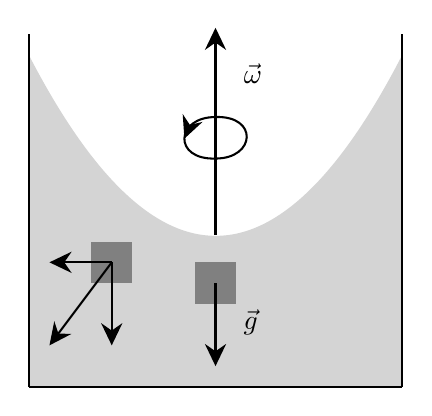
\begin{tikzpicture}[x=0.75pt,y=0.75pt,yscale=-1,xscale=1]
	%uncomment if require: \path (0,300); %set diagram left start at 0, and has height of 300

	%Shape: Polygon Curved [id:ds20096883102093122] 
	\draw  [draw opacity=0][fill={rgb, 255:red, 212; green, 212; blue, 212 }  ,fill opacity=1 ] (160,80) .. controls (220.33,196.67) and (280.33,196) .. (340,80) .. controls (340.33,162.67) and (340.33,200) .. (340,240) .. controls (278.33,239.33) and (206.33,240) .. (160,240) .. controls (160.33,198.67) and (160.33,184) .. (160,80) -- cycle ;
	%Straight Lines [id:da9654921326134607] 
	\draw    (160,70) -- (160,240) ;
	%Straight Lines [id:da6205540832353014] 
	\draw    (340,70) -- (340,240) ;
	%Straight Lines [id:da2940200728809077] 
	\draw    (160,240) -- (340,240) ;
	%Straight Lines [id:da876455808886512] 
	\draw    (250,70) -- (250,167) ;
	\draw [shift={(250,67)}, rotate = 90] [fill={rgb, 255:red, 0; green, 0; blue, 0 }  ][line width=0.08]  [draw opacity=0] (10.72,-5.15) -- (0,0) -- (10.72,5.15) -- (7.12,0) -- cycle    ;
	%Shape: Rectangle [id:dp6950850612097643] 
	\draw  [draw opacity=0][fill={rgb, 255:red, 128; green, 128; blue, 128 }  ,fill opacity=1 ] (190,170) -- (210,170) -- (210,190) -- (190,190) -- cycle ;
	%Straight Lines [id:da48466613038417683] 
	\draw    (200,217) -- (200,180) ;
	\draw [shift={(200,220)}, rotate = 270] [fill={rgb, 255:red, 0; green, 0; blue, 0 }  ][line width=0.08]  [draw opacity=0] (10.72,-5.15) -- (0,0) -- (10.72,5.15) -- (7.12,0) -- cycle    ;
	%Straight Lines [id:da4514717750458741] 
	\draw    (171.8,217.6) -- (200,180) ;
	\draw [shift={(170,220)}, rotate = 306.87] [fill={rgb, 255:red, 0; green, 0; blue, 0 }  ][line width=0.08]  [draw opacity=0] (10.72,-5.15) -- (0,0) -- (10.72,5.15) -- (7.12,0) -- cycle    ;
	%Straight Lines [id:da8756408615323261] 
	\draw    (173,180) -- (200,180) ;
	\draw [shift={(170,180)}, rotate = 0] [fill={rgb, 255:red, 0; green, 0; blue, 0 }  ][line width=0.08]  [draw opacity=0] (10.72,-5.15) -- (0,0) -- (10.72,5.15) -- (7.12,0) -- cycle    ;
	%Curve Lines [id:da4799020204729234] 
	\draw    (250,110) .. controls (230.67,110) and (229.33,130.67) .. (250,130) ;
	\draw [shift={(235,120.4)}, rotate = 291.72] [fill={rgb, 255:red, 0; green, 0; blue, 0 }  ][line width=0.08]  [draw opacity=0] (10.72,-5.15) -- (0,0) -- (10.72,5.15) -- (7.12,0) -- cycle    ;
	%Shape: Boxed Bezier Curve [id:dp013842827744275477] 
	\draw    (250.08,130) .. controls (269.41,129.93) and (270.66,109.25) .. (250,110) ;
	%Shape: Rectangle [id:dp22661450660004268] 
	\draw  [draw opacity=0][fill={rgb, 255:red, 128; green, 128; blue, 128 }  ,fill opacity=1 ] (240,180) -- (260,180) -- (260,200) -- (240,200) -- cycle ;
	%Straight Lines [id:da029217868553261583] 
	\draw    (250,227) -- (250,190) ;
	\draw [shift={(250,230)}, rotate = 270] [fill={rgb, 255:red, 0; green, 0; blue, 0 }  ][line width=0.08]  [draw opacity=0] (10.72,-5.15) -- (0,0) -- (10.72,5.15) -- (7.12,0) -- cycle    ;

	% Text Node
	\draw (268,89) node    {$\vec{\omega }$};
	% Text Node
	\draw (267,209) node    {$\vec{g}$};

	\end{tikzpicture}
\end{figure}
\FloatBarrier
La superficie andando verso il perimetro del cerchio comincia a inclinarsi e si inclina sempre di più. Si ha una parabola ruotata attorno all'asse di simmetria, che prende il nome di \emph{paraboloide di rotazione}.

\section{Il principio di Archimede}

L'ultimo concetto legato alla statica dei fluidi, è lo studio di un corpo immerso in un fluido in equilibrio statico. Si prenda un corpo di forma qualunque e lo si immerga dentro a un fluido, di densità uniforme $\rho$. Si vuole sapere se affonderà, se tenderà a galleggiare o se rimarrà in equilibrio in quel punto.

Il corpo nel fluido generalmente non rimane in equilibrio, non bisogna imporre su di esso la condizione di staticità. Si applica al centro di massa la forza peso totale. Il corpo è circondato da un fluido che genererà una pressione e quindi delle forze di superficie su ogni porzione di superficie del corpo. A esso si applica la prima equazione cardinale della dinamica: la somma vettoriale della forza peso più le forze di superficie, danno luogo alla traslazione del centro di massa del corpo.

\[
	\text{corpo:} \quad M\vec{g} + \vec{F}_s = m\vec{a}_{cm}
\]

Per risolvere questo problema bisogna capire come sono dirette e quanto sono intense le forze di superficie. Per questo si prende il fluido, si elimina il corpo e si va a considerare una porzione del fluido esattamente identifica a quella che era occupata dal solido. Tale porzione è in condizioni statiche, perché è una parte isolata di un fluido in condizioni statiche. Essa dovrà essere soggetta a una risultante delle forze che è uguale a zero, queste sono esattamente le stesse di prima: la forza peso e le forze di superficie che agiscono sulla superficie di questa porzione di fluido. Queste ultime sono le stesse che agiscono sul corpo, il fluido intorno si comporta sempre alla stessa maniera, che ci sia immerso il corpo o meno.

\begin{figure}[htpb]
	\centering

	\tikzset{every picture/.style={line width=0.75pt}} %set default line width to 0.75pt        

	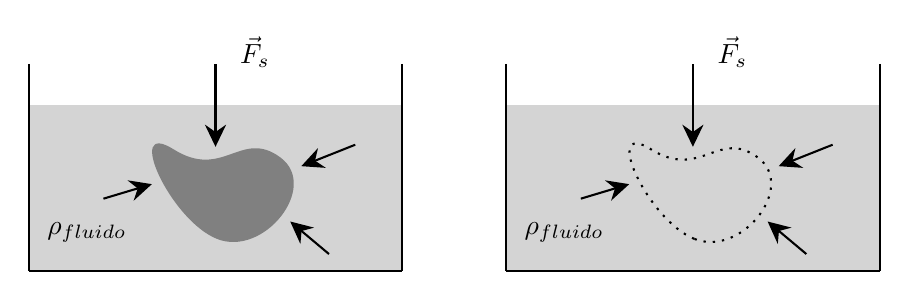
\begin{tikzpicture}[x=0.75pt,y=0.75pt,yscale=-1,xscale=1]
	%uncomment if require: \path (0,300); %set diagram left start at 0, and has height of 300

	%Shape: Rectangle [id:dp2924271807521268] 
	\draw  [draw opacity=0][fill={rgb, 255:red, 212; green, 212; blue, 212 }  ,fill opacity=1 ] (37,139) -- (217,139) -- (217,219) -- (37,219) -- cycle ;
	%Shape: Rectangle [id:dp268230096545264] 
	\draw  [draw opacity=0][fill={rgb, 255:red, 212; green, 212; blue, 212 }  ,fill opacity=1 ] (267,139) -- (447,139) -- (447,219) -- (267,219) -- cycle ;
	%Straight Lines [id:da9333188435120883] 
	\draw    (37,119) -- (37,219) ;
	%Straight Lines [id:da25664817053366384] 
	\draw    (217,119) -- (217,219) ;
	%Straight Lines [id:da8751662146914414] 
	\draw    (37,219) -- (217,219) ;
	%Straight Lines [id:da4092839702494766] 
	\draw    (127,156) -- (127,119) ;
	\draw [shift={(127,159)}, rotate = 270] [fill={rgb, 255:red, 0; green, 0; blue, 0 }  ][line width=0.08]  [draw opacity=0] (10.72,-5.15) -- (0,0) -- (10.72,5.15) -- (7.12,0) -- cycle    ;
	%Straight Lines [id:da49174964102349517] 
	\draw    (171.12,167.23) -- (194.33,158) ;
	\draw [shift={(168.33,168.33)}, rotate = 338.33] [fill={rgb, 255:red, 0; green, 0; blue, 0 }  ][line width=0.08]  [draw opacity=0] (10.72,-5.15) -- (0,0) -- (10.72,5.15) -- (7.12,0) -- cycle    ;
	%Shape: Regular Polygon [id:dp8459420545468057] 
	\draw  [draw opacity=0][fill={rgb, 255:red, 128; green, 128; blue, 128 }  ,fill opacity=1 ] (127.59,203.33) .. controls (104.98,194.13) and (82.85,145.16) .. (106.8,160.21) .. controls (130.75,175.25) and (139.36,150.04) .. (158.31,164.17) .. controls (177.27,178.31) and (150.2,212.52) .. (127.59,203.33) -- cycle ;
	%Straight Lines [id:da10166248651917864] 
	\draw    (165.3,196.93) -- (181.67,210.67) ;
	\draw [shift={(163,195)}, rotate = 40.01] [fill={rgb, 255:red, 0; green, 0; blue, 0 }  ][line width=0.08]  [draw opacity=0] (10.72,-5.15) -- (0,0) -- (10.72,5.15) -- (7.12,0) -- cycle    ;
	%Straight Lines [id:da41918106832275703] 
	\draw    (93.46,177.86) -- (73,184) ;
	\draw [shift={(96.33,177)}, rotate = 163.3] [fill={rgb, 255:red, 0; green, 0; blue, 0 }  ][line width=0.08]  [draw opacity=0] (10.72,-5.15) -- (0,0) -- (10.72,5.15) -- (7.12,0) -- cycle    ;
	%Straight Lines [id:da7859413090803753] 
	\draw    (267,119) -- (267,219) ;
	%Straight Lines [id:da8364425132614817] 
	\draw    (447,119) -- (447,219) ;
	%Straight Lines [id:da28095595212447666] 
	\draw    (267,219) -- (447,219) ;
	%Straight Lines [id:da6624570155311353] 
	\draw    (357,156) -- (357,119) ;
	\draw [shift={(357,159)}, rotate = 270] [fill={rgb, 255:red, 0; green, 0; blue, 0 }  ][line width=0.08]  [draw opacity=0] (10.72,-5.15) -- (0,0) -- (10.72,5.15) -- (7.12,0) -- cycle    ;
	%Straight Lines [id:da6892077093994595] 
	\draw    (401.12,167.23) -- (424.33,158) ;
	\draw [shift={(398.33,168.33)}, rotate = 338.33] [fill={rgb, 255:red, 0; green, 0; blue, 0 }  ][line width=0.08]  [draw opacity=0] (10.72,-5.15) -- (0,0) -- (10.72,5.15) -- (7.12,0) -- cycle    ;
	%Shape: Regular Polygon [id:dp3956362618417233] 
	\draw  [color={rgb, 255:red, 0; green, 0; blue, 0 }  ,draw opacity=1 ][dash pattern={on 0.84pt off 2.51pt}] (357.59,203.33) .. controls (334.98,194.13) and (312.85,145.16) .. (336.8,160.21) .. controls (360.75,175.25) and (369.36,150.04) .. (388.31,164.17) .. controls (407.27,178.31) and (380.2,212.52) .. (357.59,203.33) -- cycle ;
	%Straight Lines [id:da3421447885651081] 
	\draw    (395.3,196.93) -- (411.67,210.67) ;
	\draw [shift={(393,195)}, rotate = 40.01] [fill={rgb, 255:red, 0; green, 0; blue, 0 }  ][line width=0.08]  [draw opacity=0] (10.72,-5.15) -- (0,0) -- (10.72,5.15) -- (7.12,0) -- cycle    ;
	%Straight Lines [id:da6201930847496877] 
	\draw    (323.46,177.86) -- (303,184) ;
	\draw [shift={(326.33,177)}, rotate = 163.3] [fill={rgb, 255:red, 0; green, 0; blue, 0 }  ][line width=0.08]  [draw opacity=0] (10.72,-5.15) -- (0,0) -- (10.72,5.15) -- (7.12,0) -- cycle    ;

	% Text Node
	\draw (146,113.5) node    {$\vec{F}_{s}$};
	% Text Node
	\draw (65,200.17) node    {$\rho _{\text{fluido}}$};
	% Text Node
	\draw (376,113.5) node    {$\vec{F}_{s}$};
	% Text Node
	\draw (295,200.17) node    {$\rho _{\text{fluido}}$};

	\end{tikzpicture}
\end{figure}
\FloatBarrier
Quindi:

\[
	\text{fluido:} \quad M_{\text{fluido} }\vec{g} +\vec{F}_s = 0 \implies \vec{F}_s = -M_{\text{fluido} }\vec{g} = -\rho_{\text{fluido} }V\vec{g}
\]

Si indica un versore $\vec{u}_z$ diretto verso l'alto.

\[
	\vec{F}_s = \rho_{\text{fluido} }Vg\vec{u}_z = \vec{F}_{\text{Archimede} }
\]

Questa quantità si chiama \textbf{spinta di Archimede}. Il \textbf{principio di Archimede} afferma che quando si ha un corpo immerso in un fluido, questo riceve una spinta verso l'alto di intensità pari al peso del volume di fluido occupata dal corpo. Il volume sarà solo la porzione immersa nel fluido perché si trascura la spinta di Archimede dell' atmosfera. Invece di disegnare tutte le forze di superficie, se ne disegna la risultante: è una forza diretta come $\vec{g}$ ma verso l'alto. Se la spinta di Archimede è minore del peso il corpo affonda. Se le due cose sono uguali il corpo fluttua. Se essa è invece maggiore del peso, il corpo galleggia.
Si dimostra che la spinta di Archimede, essendo in generale i corpi esterni estesi, si applica nel centro di massa della parte immersa. Solo se tutto il corpo è immerso, esso coincide con il baricentro del corpo.

\begin{gather*}
	\text{corpo tutto immerso:} \quad M\vec{g} +\vec{F}_s = M\vec{a}_{cm} \\
	-\rho Vg\vec{u}_z + \rho_{\text{fluido} }Vg\vec{u}_z = (\rho_{\text{fluido} }- \rho)Vg\vec{u}_z
\end{gather*}

Si ottiene che il corpo si muoverà verso l'alto.

\[
	\rho_{\text{fluido} }-\rho \left\{ \begin{array}{l}
	 	\rho > \rho_{\text{fluido}} \implies \text{il corpo affonda} \\
	 	\rho = \rho_{\text{fluido}} \implies \text{il corpo fluttua} \\
	 	\rho < \rho_{\text{fluido}} \implies \text{il corpo galleggia} \\
	\end{array} \right.
\]

Il fatto che il corpo galleggi significa che esso, totalmente immerso, risale verso l'alto fino a quando la spinta di Archimede non arriva a bilanciare la forza peso. La spinta di Archimede diminuisce perché quando il corpo incomincia a fuoriuscire dall'acqua diminuisce il volume immerso.

\[
	-\rho Vg\vec{u}_z + \rho_{\text{fluido} }\widetilde{V}g\vec{u}_z=0
\]

Non solo le forze si devono bilanciare fra di loro, ma si devono bilanciare anche i momenti delle forze. Questa è una condizione necessaria per il galleggiamento delle barche. Quando soltanto una parte del corpo galleggia, il baricentro del corpo e quello della parte immersa non coincidono, il loro momento è zero finché si trovano sulla stessa retta parallela a $\vec{g}$.
Quando la barca si inclina, ad esempio a causa delle onde, gli scafi delle barche devono essere progettati in maniera tale che essa reagisca riportandosi in posizione di equilibrio (si veda la figura).

\begin{figure}[htpb]
	\centering

	% Pattern Info
	 
	\tikzset{
	pattern size/.store in=\mcSize, 
	pattern size = 5pt,
	pattern thickness/.store in=\mcThickness, 
	pattern thickness = 0.3pt,
	pattern radius/.store in=\mcRadius, 
	pattern radius = 1pt}
	\makeatletter
	\pgfutil@ifundefined{pgf@pattern@name@_31vtuqmc4}{
	\pgfdeclarepatternformonly[\mcThickness,\mcSize]{_31vtuqmc4}
	{\pgfqpoint{0pt}{0pt}}
	{\pgfpoint{\mcSize+\mcThickness}{\mcSize+\mcThickness}}
	{\pgfpoint{\mcSize}{\mcSize}}
	{
	\pgfsetcolor{\tikz@pattern@color}
	\pgfsetlinewidth{\mcThickness}
	\pgfpathmoveto{\pgfqpoint{0pt}{0pt}}
	\pgfpathlineto{\pgfpoint{\mcSize+\mcThickness}{\mcSize+\mcThickness}}
	\pgfusepath{stroke}
	}}
	\makeatother

	% Pattern Info
	 
	\tikzset{
	pattern size/.store in=\mcSize, 
	pattern size = 5pt,
	pattern thickness/.store in=\mcThickness, 
	pattern thickness = 0.3pt,
	pattern radius/.store in=\mcRadius, 
	pattern radius = 1pt}
	\makeatletter
	\pgfutil@ifundefined{pgf@pattern@name@_q84sces0b}{
	\pgfdeclarepatternformonly[\mcThickness,\mcSize]{_q84sces0b}
	{\pgfqpoint{0pt}{0pt}}
	{\pgfpoint{\mcSize+\mcThickness}{\mcSize+\mcThickness}}
	{\pgfpoint{\mcSize}{\mcSize}}
	{
	\pgfsetcolor{\tikz@pattern@color}
	\pgfsetlinewidth{\mcThickness}
	\pgfpathmoveto{\pgfqpoint{0pt}{0pt}}
	\pgfpathlineto{\pgfpoint{\mcSize+\mcThickness}{\mcSize+\mcThickness}}
	\pgfusepath{stroke}
	}}
	\makeatother
	\tikzset{every picture/.style={line width=0.75pt}} %set default line width to 0.75pt        

	\begin{tikzpicture}[x=0.75pt,y=0.75pt,yscale=-1,xscale=1]
	%uncomment if require: \path (0,300); %set diagram left start at 0, and has height of 300

	%Shape: Rectangle [id:dp47829763359688604] 
	\draw  [draw opacity=0][fill={rgb, 255:red, 212; green, 212; blue, 212 }  ,fill opacity=1 ] (70.5,141) -- (269.5,141) -- (269.5,201) -- (70.5,201) -- cycle ;
	%Flowchart: Delay [id:dp29197696959440433] 
	\draw  [color={rgb, 255:red, 128; green, 128; blue, 128 }  ,draw opacity=1 ][fill={rgb, 255:red, 128; green, 128; blue, 128 }  ,fill opacity=1 ] (215,123.67) -- (215,149) .. controls (215,162.99) and (194.78,174.33) .. (169.83,174.33) .. controls (144.89,174.33) and (124.67,162.99) .. (124.67,149) -- (124.67,123.67) -- cycle ;
	%Shape: Circle [id:dp8821713706044376] 
	\draw  [fill={rgb, 255:red, 0; green, 0; blue, 0 }  ,fill opacity=1 ] (167.33,153.5) .. controls (167.33,152.12) and (168.45,151) .. (169.83,151) .. controls (171.21,151) and (172.33,152.12) .. (172.33,153.5) .. controls (172.33,154.88) and (171.21,156) .. (169.83,156) .. controls (168.45,156) and (167.33,154.88) .. (167.33,153.5) -- cycle ;
	%Curve Lines [id:da7112974575143318] 
	\draw    (175.62,93.91) .. controls (201.37,86.54) and (231.23,100.38) .. (237.82,125.8) ;
	\draw [shift={(238.44,128.61)}, rotate = 259.51] [fill={rgb, 255:red, 0; green, 0; blue, 0 }  ][line width=0.08]  [draw opacity=0] (10.72,-5.15) -- (0,0) -- (10.72,5.15) -- (7.12,0) -- cycle    ;
	%Straight Lines [id:da2837377357891766] 
	\draw    (70.5,131) -- (70.5,201) ;
	%Straight Lines [id:da2684328230332256] 
	\draw    (269.5,131) -- (269.5,201) ;
	%Straight Lines [id:da7800389284596869] 
	\draw    (269.5,201) -- (70.5,201) ;
	%Shape: Path Data [id:dp45697782539174714] 
	\draw  [color={rgb, 255:red, 0; green, 0; blue, 0 }  ,draw opacity=1 ][pattern=_31vtuqmc4,pattern size=6pt,pattern thickness=0.75pt,pattern radius=0pt, pattern color={rgb, 255:red, 0; green, 0; blue, 0}] (215,149) .. controls (215,162.99) and (194.78,174.33) .. (169.83,174.33) .. controls (144.89,174.33) and (124.67,162.99) .. (124.67,149) -- (124.67,141) -- (215,141) -- (215,149) -- cycle ;
	%Shape: Circle [id:dp30364608297317264] 
	\draw  [fill={rgb, 255:red, 0; green, 0; blue, 0 }  ,fill opacity=1 ] (167.33,133.5) .. controls (167.33,132.12) and (168.45,131) .. (169.83,131) .. controls (171.21,131) and (172.33,132.12) .. (172.33,133.5) .. controls (172.33,134.88) and (171.21,136) .. (169.83,136) .. controls (168.45,136) and (167.33,134.88) .. (167.33,133.5) -- cycle ;
	%Shape: Rectangle [id:dp2713282993239199] 
	\draw  [draw opacity=0][fill={rgb, 255:red, 212; green, 212; blue, 212 }  ,fill opacity=1 ] (319.5,141) -- (518.5,141) -- (518.5,201) -- (319.5,201) -- cycle ;
	%Flowchart: Delay [id:dp4272201970702536] 
	\draw  [color={rgb, 255:red, 128; green, 128; blue, 128 }  ,draw opacity=1 ][fill={rgb, 255:red, 128; green, 128; blue, 128 }  ,fill opacity=1 ] (470.58,148.92) -- (459.08,171.49) .. controls (452.74,183.96) and (429.57,184.89) .. (407.34,173.58) .. controls (385.11,162.26) and (372.23,142.98) .. (378.58,130.51) -- (390.08,107.93) -- cycle ;
	%Curve Lines [id:da141599797063642] 
	\draw    (434.84,89.44) .. controls (460.75,83.83) and (489.61,98.83) .. (494.44,124.94) ;
	\draw [shift={(431.62,90.25)}, rotate = 344.02] [fill={rgb, 255:red, 0; green, 0; blue, 0 }  ][line width=0.08]  [draw opacity=0] (10.72,-5.15) -- (0,0) -- (10.72,5.15) -- (7.12,0) -- cycle    ;
	%Straight Lines [id:da26918340914974825] 
	\draw    (319.5,131) -- (319.5,201) ;
	%Straight Lines [id:da6034750913598959] 
	\draw    (518.5,131) -- (518.5,201) ;
	%Straight Lines [id:da3957935253978764] 
	\draw    (518.5,201) -- (319.5,201) ;
	%Shape: Circle [id:dp23398629144511873] 
	\draw  [fill={rgb, 255:red, 0; green, 0; blue, 0 }  ,fill opacity=1 ] (417.9,152.7) .. controls (418.63,151.69) and (420.05,151.46) .. (421.06,152.19) .. controls (422.08,152.93) and (422.31,154.34) .. (421.57,155.36) .. controls (420.84,156.37) and (419.42,156.6) .. (418.41,155.87) .. controls (417.39,155.14) and (417.16,153.72) .. (417.9,152.7) -- cycle ;
	%Shape: Circle [id:dp8816370101911546] 
	\draw  [fill={rgb, 255:red, 0; green, 0; blue, 0 }  ,fill opacity=1 ] (428.61,161.24) .. controls (429.32,160.24) and (430.71,160.02) .. (431.7,160.74) .. controls (432.69,161.45) and (432.91,162.84) .. (432.2,163.83) .. controls (431.48,164.82) and (430.1,165.04) .. (429.11,164.33) .. controls (428.11,163.61) and (427.89,162.23) .. (428.61,161.24) -- cycle ;
	%Straight Lines [id:da38157126120264007] 
	\draw    (419.74,191.03) -- (419.74,154.03) ;
	\draw [shift={(419.74,194.03)}, rotate = 270] [fill={rgb, 255:red, 0; green, 0; blue, 0 }  ][line width=0.08]  [draw opacity=0] (10.72,-5.15) -- (0,0) -- (10.72,5.15) -- (7.12,0) -- cycle    ;
	%Straight Lines [id:da36464594177504006] 
	\draw    (430.4,162.53) -- (430.4,125.53) ;
	\draw [shift={(430.4,122.53)}, rotate = 450] [fill={rgb, 255:red, 0; green, 0; blue, 0 }  ][line width=0.08]  [draw opacity=0] (10.72,-5.15) -- (0,0) -- (10.72,5.15) -- (7.12,0) -- cycle    ;
	%Shape: Path Data [id:dp5684196922078801] 
	\draw  [color={rgb, 255:red, 0; green, 0; blue, 0 }  ,draw opacity=1 ][pattern=_q84sces0b,pattern size=6pt,pattern thickness=0.75pt,pattern radius=0pt, pattern color={rgb, 255:red, 0; green, 0; blue, 0}] (459.08,171.49) .. controls (452.74,183.96) and (429.57,184.89) .. (407.34,173.58) .. controls (390.71,165.11) and (379.32,152.19) .. (377.29,141) -- (455.03,141) -- (470.58,148.92) ;

	% Text Node
	\draw (396.67,184.83) node    {$M\vec{g}$};
	% Text Node
	\draw (446.67,112.83) node    {$\vec{F}_{A}$};

	\end{tikzpicture}
\end{figure}
\FloatBarrier
Questo si verifica se la spinta di Archimede tende a far ruotare la barca in senso opposto a quello della perturbazione compensando lo sbilanciamento.

\begin{figure}[htpb]
	\centering

	% Pattern Info
	 
	\tikzset{
	pattern size/.store in=\mcSize, 
	pattern size = 5pt,
	pattern thickness/.store in=\mcThickness, 
	pattern thickness = 0.3pt,
	pattern radius/.store in=\mcRadius, 
	pattern radius = 1pt}
	\makeatletter
	\pgfutil@ifundefined{pgf@pattern@name@_v6p0c9ovg}{
	\pgfdeclarepatternformonly[\mcThickness,\mcSize]{_v6p0c9ovg}
	{\pgfqpoint{0pt}{0pt}}
	{\pgfpoint{\mcSize+\mcThickness}{\mcSize+\mcThickness}}
	{\pgfpoint{\mcSize}{\mcSize}}
	{
	\pgfsetcolor{\tikz@pattern@color}
	\pgfsetlinewidth{\mcThickness}
	\pgfpathmoveto{\pgfqpoint{0pt}{0pt}}
	\pgfpathlineto{\pgfpoint{\mcSize+\mcThickness}{\mcSize+\mcThickness}}
	\pgfusepath{stroke}
	}}
	\makeatother

	% Pattern Info
	 
	\tikzset{
	pattern size/.store in=\mcSize, 
	pattern size = 5pt,
	pattern thickness/.store in=\mcThickness, 
	pattern thickness = 0.3pt,
	pattern radius/.store in=\mcRadius, 
	pattern radius = 1pt}
	\makeatletter
	\pgfutil@ifundefined{pgf@pattern@name@_xvr8v4s9a}{
	\pgfdeclarepatternformonly[\mcThickness,\mcSize]{_xvr8v4s9a}
	{\pgfqpoint{0pt}{0pt}}
	{\pgfpoint{\mcSize+\mcThickness}{\mcSize+\mcThickness}}
	{\pgfpoint{\mcSize}{\mcSize}}
	{
	\pgfsetcolor{\tikz@pattern@color}
	\pgfsetlinewidth{\mcThickness}
	\pgfpathmoveto{\pgfqpoint{0pt}{0pt}}
	\pgfpathlineto{\pgfpoint{\mcSize+\mcThickness}{\mcSize+\mcThickness}}
	\pgfusepath{stroke}
	}}
	\makeatother
	\tikzset{every picture/.style={line width=0.75pt}} %set default line width to 0.75pt        

	\begin{tikzpicture}[x=0.75pt,y=0.75pt,yscale=-1,xscale=1]
	%uncomment if require: \path (0,300); %set diagram left start at 0, and has height of 300

	%Shape: Rectangle [id:dp9862095167922351] 
	\draw  [draw opacity=0][fill={rgb, 255:red, 212; green, 212; blue, 212 }  ,fill opacity=1 ] (296.5,160) -- (463.5,160) -- (463.5,220) -- (296.5,220) -- cycle ;
	%Straight Lines [id:da447179809049856] 
	\draw    (296.5,150) -- (296.5,220) ;
	%Straight Lines [id:da3781711975130897] 
	\draw    (463.5,150) -- (463.5,220) ;
	%Straight Lines [id:da9710787433089609] 
	\draw    (463.5,220) -- (296.5,220) ;
	%Flowchart: Delay [id:dp34858695131676476] 
	\draw  [color={rgb, 255:red, 128; green, 128; blue, 128 }  ,draw opacity=1 ][fill={rgb, 255:red, 128; green, 128; blue, 128 }  ,fill opacity=1 ] (417.15,148.4) -- (396.66,176.78) .. controls (385.35,192.45) and (370.73,201.23) .. (364.01,196.38) .. controls (357.3,191.53) and (361.02,174.89) .. (372.34,159.22) -- (392.83,130.84) -- cycle ;
	%Shape: Circle [id:dp47969536261711365] 
	\draw  [fill={rgb, 255:red, 0; green, 0; blue, 0 }  ,fill opacity=1 ] (384.56,164.04) .. controls (385.3,163.02) and (386.71,162.79) .. (387.73,163.53) .. controls (388.75,164.26) and (388.97,165.68) .. (388.24,166.69) .. controls (387.51,167.71) and (386.09,167.94) .. (385.08,167.2) .. controls (384.06,166.47) and (383.83,165.05) .. (384.56,164.04) -- cycle ;
	%Shape: Circle [id:dp9500480670392788] 
	\draw  [fill={rgb, 255:red, 0; green, 0; blue, 0 }  ,fill opacity=1 ] (375.61,176.57) .. controls (376.32,175.58) and (377.71,175.35) .. (378.7,176.07) .. controls (379.69,176.79) and (379.91,178.17) .. (379.2,179.16) .. controls (378.48,180.15) and (377.1,180.38) .. (376.11,179.66) .. controls (375.11,178.94) and (374.89,177.56) .. (375.61,176.57) -- cycle ;
	%Straight Lines [id:da4084746695198622] 
	\draw    (386.4,202.37) -- (386.4,165.37) ;
	\draw [shift={(386.4,205.37)}, rotate = 270] [fill={rgb, 255:red, 0; green, 0; blue, 0 }  ][line width=0.08]  [draw opacity=0] (10.72,-5.15) -- (0,0) -- (10.72,5.15) -- (7.12,0) -- cycle    ;
	%Straight Lines [id:da608832121120398] 
	\draw    (377.4,177.87) -- (377.4,140.87) ;
	\draw [shift={(377.4,137.87)}, rotate = 450] [fill={rgb, 255:red, 0; green, 0; blue, 0 }  ][line width=0.08]  [draw opacity=0] (10.72,-5.15) -- (0,0) -- (10.72,5.15) -- (7.12,0) -- cycle    ;
	%Curve Lines [id:da11003730679167623] 
	\draw    (370.29,97.91) .. controls (396.04,90.54) and (425.9,104.38) .. (432.48,129.8) ;
	\draw [shift={(433.11,132.61)}, rotate = 259.51] [fill={rgb, 255:red, 0; green, 0; blue, 0 }  ][line width=0.08]  [draw opacity=0] (10.72,-5.15) -- (0,0) -- (10.72,5.15) -- (7.12,0) -- cycle    ;
	%Shape: Path Data [id:dp8117456064987676] 
	\draw  [color={rgb, 255:red, 0; green, 0; blue, 0 }  ,draw opacity=1 ][pattern=_v6p0c9ovg,pattern size=6pt,pattern thickness=0.75pt,pattern radius=0pt, pattern color={rgb, 255:red, 0; green, 0; blue, 0}] (396.66,176.78) .. controls (385.35,192.45) and (370.73,201.23) .. (364.01,196.38) .. controls (357.41,191.61) and (360.9,175.44) .. (371.78,160) -- (408.78,160) -- (396.66,176.78) -- cycle ;
	%Shape: Rectangle [id:dp7984287448127838] 
	\draw  [draw opacity=0][fill={rgb, 255:red, 212; green, 212; blue, 212 }  ,fill opacity=1 ] (79.5,160) -- (246.5,160) -- (246.5,220) -- (79.5,220) -- cycle ;
	%Flowchart: Delay [id:dp9187309202524181] 
	\draw  [color={rgb, 255:red, 128; green, 128; blue, 128 }  ,draw opacity=1 ][fill={rgb, 255:red, 128; green, 128; blue, 128 }  ,fill opacity=1 ] (176,130) -- (176,165) .. controls (176,184.33) and (169.28,200) .. (161,200) .. controls (152.72,200) and (146,184.33) .. (146,165) -- (146,130) -- cycle ;
	%Shape: Circle [id:dp9403857998134741] 
	\draw  [fill={rgb, 255:red, 0; green, 0; blue, 0 }  ,fill opacity=1 ] (158.5,161.75) .. controls (158.5,160.37) and (159.62,159.25) .. (161,159.25) .. controls (162.38,159.25) and (163.5,160.37) .. (163.5,161.75) .. controls (163.5,163.13) and (162.38,164.25) .. (161,164.25) .. controls (159.62,164.25) and (158.5,163.13) .. (158.5,161.75) -- cycle ;
	%Curve Lines [id:da5917708601819769] 
	\draw    (132.29,97.91) .. controls (158.04,90.54) and (187.9,104.38) .. (194.48,129.8) ;
	\draw [shift={(195.11,132.61)}, rotate = 259.51] [fill={rgb, 255:red, 0; green, 0; blue, 0 }  ][line width=0.08]  [draw opacity=0] (10.72,-5.15) -- (0,0) -- (10.72,5.15) -- (7.12,0) -- cycle    ;
	%Straight Lines [id:da4782038123895451] 
	\draw    (79.5,150) -- (79.5,220) ;
	%Straight Lines [id:da039222109655102866] 
	\draw    (246.5,150) -- (246.5,220) ;
	%Straight Lines [id:da352891107189514] 
	\draw    (246.5,220) -- (79.5,220) ;
	%Shape: Path Data [id:dp5449531698933052] 
	\draw  [color={rgb, 255:red, 0; green, 0; blue, 0 }  ,draw opacity=1 ][pattern=_xvr8v4s9a,pattern size=6pt,pattern thickness=0.75pt,pattern radius=0pt, pattern color={rgb, 255:red, 0; green, 0; blue, 0}] (176,165) .. controls (176,184.33) and (169.28,200) .. (161,200) .. controls (152.72,200) and (146,184.33) .. (146,165) -- (146,160) -- (176,160) -- (176,165) -- cycle ;

	% Text Node
	\draw (360.67,128.83) node    {$\vec{F}_{A}$};
	% Text Node
	\draw (409.67,197.83) node    {$M\vec{g}$};

	\end{tikzpicture}
\end{figure}
\FloatBarrier
Se si ha uno scafo molto più lungo e molto più stretto, la parte immersa è un po' più spostata verso sinistra. Uno scafo di questo tipo tende a ribaltare ulteriormente la barca.